% g6e_H.tex — 6thGradeReviewExplanations, pp. 12–22:
% Section D (D1–D4), Section E (E1–E4), Section F (F1–F6).
% Fragment: \input into a wrapper that loads mathdocs.sty.

% ---------------------------------------------------------------------------
\lesson{D. Facts And Decimal Multiply/Divide}

\question{D1}

\blockhead{Question}
\noindent $9 \times 6 = $

\checked{$54$}

\blockhead{What the question is asking}
\noindent This question asks for the answer when you multiply $9$ and $6$.

\blockhead{Important words}
\begin{words}
  \item \term{Multiply}means find a total of equal groups.
  \item The \term{product}is the answer to a multiplication problem.
  \item A \term{factor}is a number being multiplied. Here the factors are $9$ and $6$.
  \item Equal groups: $9$ groups of $6$ means $6 + 6 + 6 + 6 + 6 + 6 + 6 + 6 + 6$.
\end{words}

\blockhead{Work the problem one tiny step at a time}
\begin{steps}
  \item Think of $9$ groups of $6$, or $6$ groups of $9$.
  \item Use a known fact: $9 \times 5 = 45$.
  \item Add one more group of $9$: $45 + 9 = 54$.
  \item Another path: $10 \times 6 = 60$, then take away one $6$: $60 - 6 = 54$.
  \item Check by dividing: $54 \div 9 = 6$ (because $9 \times 6 = 54$).
\end{steps}

\finalans{$54$}

\blockhead{Why this makes sense}
\noindent Check with addition: $6 + 6 + 6 + 6 + 6 + 6 + 6 + 6 + 6 = 54$. Or
check $54 \div 9 = 6$.

% ---------------------------------------------------------------------------
\question{D2}

\blockhead{Question}
\noindent $63 \div 9 = $

\checked{$7$}

\blockhead{What the question is asking}
\noindent This question asks how many times $9$ fits into $63$.

\blockhead{Important words}
\begin{words}
  \item \term{Divide}means split into equal groups.
  \item The \term{quotient}is the answer to a division problem.
  \item The \term{dividend}is the number being divided ($63$).
  \item The \term{divisor}is the number you divide by ($9$).
  \item Division undoes multiplication: if $9 \times 7 = 63$, then $63 \div 9 = 7$.
\end{words}

\blockhead{Work the problem one tiny step at a time}
\begin{steps}
  \item Ask: what times $9$ equals $63$?
  \item Try $9 \times 6$: $9 \times 6 = 54$. That is less than $63$, so try one more.
  \item Try $9 \times 7$: $9 \times 7 = 63$. Exact match.
  \item So $63 \div 9 = 7$.
  \item Check: multiply back --- $9 \times 7 = 63$.
\end{steps}

\finalans{$7$}

\blockhead{Why this makes sense}
\noindent Multiplication check: $9 \times 7 = 63$. The quotient must be $7$.

% ---------------------------------------------------------------------------
\question{D3}

\blockhead{Question}
\noindent $2.4 \times 1.5 = $\blank\hint{decimal}

\checked{$3.6$}

\blockhead{What the question is asking}
\noindent This question asks you to multiply two numbers that use a dot for
parts of a whole.

\blockhead{Important words}
\begin{words}
  \item A \term{factor}is a number being multiplied. Here the factors are $2.4$ and $1.5$.
  \item A \term{decimal digit}is a digit to the right of the decimal point (after the dot).
  \item To multiply decimals: multiply as if they were whole numbers, then place the
        decimal point by counting all decimal digits in the factors.
\end{words}

\blockhead{Work the problem one tiny step at a time}
\begin{steps}
  \item Ignore the points for a moment: multiply $24 \times 15$.
  \item $24 \times 10 = 240$.
  \item $24 \times 5 = 120$.
  \item Add: $240 + 120 = 360$.
  \item Count decimal digits: $2.4$ has $1$ digit after the point; $1.5$ has $1$ digit
        after the point; total $2$ digits.
  \item Place the point two places from the right in $360$: $3.60$.
  \item You may drop the trailing zero: $3.60 = 3.6$.
\end{steps}

\finalans{$3.6$}

\blockhead{Why this makes sense}
\noindent Estimate: $2 \times 1.5 = 3$, and $2.4$ is a bit more than $2$, so
about $3.6$ makes sense.

% ---------------------------------------------------------------------------
\question{D4}

\blockhead{Question}
\noindent $5.6 \div 0.8 = $\blank

\checked{$7$}

\blockhead{What the question is asking}
\noindent This question asks you to divide $5.6$ by $0.8$.

\blockhead{Important words}
\begin{words}
  \item The \term{dividend}is the number being divided ($5.6$).
  \item The \term{divisor}is the number you divide by ($0.8$).
  \item The \term{quotient}is the answer to a division problem.
  \item A \term{power of ten}is a number like $10$, $100$, or $1000$ made by
        multiplying tens together.
  \item To divide by a decimal, multiply the dividend and the divisor by the same
        power of ten so the divisor becomes a whole number.
\end{words}

\blockhead{Work the problem one tiny step at a time}
\begin{steps}
  \item Name the parts: dividend $5.6$, divisor $0.8$.
  \item Multiply both $5.6$ and $0.8$ by $10$ to clear one decimal place in the divisor.
  \item $5.6 \times 10 = 56$ and $0.8 \times 10 = 8$.
  \item Now compute $56 \div 8$.
  \item $8 \times 7 = 56$, so $56 \div 8 = 7$.
  \item Therefore $5.6 \div 0.8 = 7$.
\end{steps}

\finalans{$7$}

\blockhead{Why this makes sense}
\noindent Check: $0.8 \times 7 = 5.6$. Yes, the quotient $7$ is correct.

% ---------------------------------------------------------------------------
\lesson{E. Ratios, Fractions, And Proportions}

\question{E1}

\blockhead{Question}
\noindent Greater: $\dfrac{5}{8}$ or $0.61$?

\checked{$\dfrac{5}{8}$}

\blockhead{What the question is asking}
\noindent This question asks which number is larger: $\dfrac{5}{8}$ or $0.61$.

\blockhead{Important words}
\begin{words}
  \item To \term{compare}a fraction and a decimal, write both in the same form
        (both decimals or both fractions).
  \item A \term{fraction bar}means divide: $\dfrac{5}{8}$ means $5 \div 8$.
  \item A \term{remainder}is what is left over after a division step (how much is
        still not divided).
  \item To \term{bring down}a digit means move the next digit (often a $0$ after the
        decimal) into the current remainder so you can keep dividing.
\end{words}

\blockhead{Work the problem one tiny step at a time}
\begin{steps}
  \item Change $\dfrac{5}{8}$ to a decimal by dividing $5 \div 8$.
  \item $8$ into $50$ is $6$ (because $8 \times 6 = 48$), remainder $2$.
  \item Bring down $0$: $20 \div 8 = 2$ (because $8 \times 2 = 16$), remainder $4$.
  \item Bring down $0$: $40 \div 8 = 5$. So $5 \div 8 = 0.625$.
  \item Compare $0.625$ and $0.61$. Line up: $0.625$ versus $0.610$.
  \item Tenths: both have $6$. Hundredths: $2 > 1$, so $0.625 > 0.610$ already
        (thousandths $5 > 0$ also agrees).
  \item Therefore $\dfrac{5}{8}$ is greater.
\end{steps}

\finalans{$\dfrac{5}{8}$}

\blockhead{Why this makes sense}
\noindent $0.625$ is a little more than $0.61$ because the hundredths digit $2$
beats $1$. So the fraction $\dfrac{5}{8}$ wins.

% ---------------------------------------------------------------------------
\question{E2}

\blockhead{Question}
\[ \frac{4}{7} = \frac{?}{21} \]

\checked{$12$}

\blockhead{What the question is asking}
\noindent This question asks for the missing top number that makes the two
equal-parts-over-a-whole amounts equal.

\blockhead{Important words}
\begin{words}
  \item \term{Equal fractions}name the same amount, even if the numbers look different.
  \item A \term{ratio}compares two amounts. You can write a ratio as a fraction,
        like $\dfrac{4}{7}$.
  \item An \term{equation}is a math sentence with an equals sign that says two sides
        are equal.
  \item A \term{proportion}is an equation that says two ratios (fractions) are equal.
  \item The \term{butterfly method}(cross multiply) multiplies along the diagonals of
        two equal fractions.
  \item \term{Cross products}are the two diagonal products from the butterfly
        ($a \times d$ and $b \times c$).
  \item The \term{numerator}is the top. The \term{denominator}is the bottom.
\end{words}

\blockhead{Work the problem one tiny step at a time}
\begin{steps}
  \item Write the equal fractions: $\dfrac{4}{7} = \dfrac{?}{21}$.
  \item Draw the butterfly (cross-multiply picture) below.
  \item Cross multiply along the red lines: $4 \times 21 = 7 \times {?}$.
  \item Compute $4 \times 21$: $4 \times 20 = 80$ and $4 \times 1 = 4$, so $84$.
  \item So $84 = 7 \times {?}$.
  \item Divide both sides by $7$ (shown under the equals):
    \begin{center}
      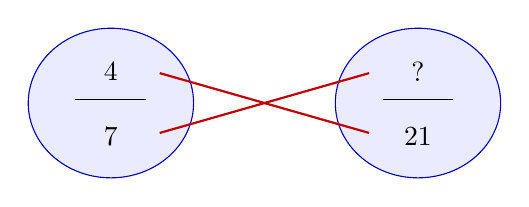
\begin{tikzpicture}[x=1cm,y=1cm]
        \fill[blue!8] (0,0) ellipse (1.05 and 0.95);
        \draw[blue!70!black] (0,0) ellipse (1.05 and 0.95);
        \fill[blue!8] (3.9,0) ellipse (1.05 and 0.95);
        \draw[blue!70!black] (3.9,0) ellipse (1.05 and 0.95);
        \draw[red!75!black,thick] (0.62,0.38) -- (3.28,-0.38);
        \draw[red!75!black,thick] (0.62,-0.38) -- (3.28,0.38);
        \node at (0,0.40) {$4$};
        \draw (-0.45,0.05) -- (0.45,0.05);
        \node at (0,-0.42) {$7$};
        \node at (3.9,0.40) {$?$};
        \draw (3.45,0.05) -- (4.35,0.05);
        \node at (3.9,-0.42) {$21$};
      \end{tikzpicture}
      \par\smallskip
      Butterfly: multiply along each red line.
      \par\medskip
      $84 = 7 \times {?}$
      \par\smallskip
      \underline{\textcolor{blue!60!black}{$\div 7$\qquad$\div 7$}}
    \end{center}
  \item Compute the leftover division: $84 \div 7 = 12$ (because $7 \times 12 = 84$).
  \item So ${?} = 12$.
\end{steps}

\finalans{$12$}

\blockhead{Why this makes sense}
\noindent Check another way: $7 \times 3 = 21$, so multiply the top by the same
$3$: $4 \times 3 = 12$. Same answer. Cross products match: $4 \times 21 = 84$
and $7 \times 12 = 84$.

% ---------------------------------------------------------------------------
\question{E3}

\blockhead{Question}
\noindent $4$ snacks cost \money{20}. $7$ snacks cost \blank[2.4cm]\ dollars.

\checked{$35$ dollars}

\blockhead{What the question is asking}
\noindent This question asks how many dollars $7$ snacks cost if $4$ snacks
cost \money{20} and the price stays in the same pattern.

\blockhead{Important words}
\begin{words}
  \item A \term{ratio}compares two amounts (here, snacks to dollars).
  \item A \term{proportion}keeps two ratios equal.
  \item A \term{unit price}is the cost of one item.
  \item We use the butterfly (cross multiply) when two fractions are equal.
\end{words}

\blockhead{Work the problem one tiny step at a time}
\begin{steps}
  \item Set up a proportion. Keep snacks on top and dollars on bottom (or keep the
        same order on both sides).
  \item One correct setup:
    \[ \frac{4\ \text{snacks}}{20\ \text{dollars}} = \frac{7\ \text{snacks}}{x\ \text{dollars}} \]
  \item Draw the butterfly and cross multiply: $4 \times x = 20 \times 7$.
  \item Break $20 \times 7$: $20 \times 5 = 100$ and $20 \times 2 = 40$, then
        $100 + 40 = 140$.
  \item So $4x = 140$.
  \item Divide both sides by $4$:
    \begin{center}
      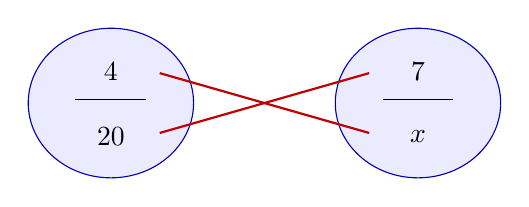
\begin{tikzpicture}[x=1cm,y=1cm]
        \fill[blue!8] (0,0) ellipse (1.05 and 0.95);
        \draw[blue!70!black] (0,0) ellipse (1.05 and 0.95);
        \fill[blue!8] (3.9,0) ellipse (1.05 and 0.95);
        \draw[blue!70!black] (3.9,0) ellipse (1.05 and 0.95);
        \draw[red!75!black,thick] (0.62,0.38) -- (3.28,-0.38);
        \draw[red!75!black,thick] (0.62,-0.38) -- (3.28,0.38);
        \node at (0,0.40) {$4$};
        \draw (-0.45,0.05) -- (0.45,0.05);
        \node at (0,-0.42) {$20$};
        \node at (3.9,0.40) {$7$};
        \draw (3.45,0.05) -- (4.35,0.05);
        \node at (3.9,-0.42) {$x$};
      \end{tikzpicture}
      \par\smallskip
      Butterfly: multiply along each red line.
      \par\medskip
      $4x = 140$
      \par\smallskip
      \underline{\textcolor{blue!60!black}{$\div 4$\qquad$\div 4$}}
    \end{center}
  \item Compute the leftover division: $140 \div 4 = 35$ (because
        $4 \times 35 = 140$).
  \item So $x = 35$.
\end{steps}

\finalans{$35$ dollars}

\blockhead{Why this makes sense}
\noindent Unit-price check: one snack costs $20 \div 4 = 5$ dollars. Then $7$
snacks cost $7 \times 5 = 35$ dollars. Same answer.

% ---------------------------------------------------------------------------
\question{E4}

\blockhead{Question}
\[ \frac{5}{6} = \frac{x}{18} \]

\checked{$x = 15$}

\blockhead{What the question is asking}
\noindent This question asks for the value of $x$ that makes the two
equal-parts-over-a-whole amounts equal.

\blockhead{Important words}
\begin{words}
  \item $x$ is a \term{variable}: a letter that stands for an unknown number.
  \item Use the \term{butterfly method}(cross multiply) for equal fractions.
\end{words}

\blockhead{Work the problem one tiny step at a time}
\begin{steps}
  \item Write $\dfrac{5}{6} = \dfrac{x}{18}$.
  \item Cross multiply: $5 \times 18 = 6 \times x$.
  \item Compute $5 \times 18 = 90$.
  \item So $90 = 6x$.
  \item Divide both sides by $6$:
    \begin{center}
      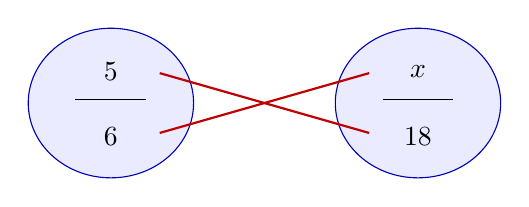
\begin{tikzpicture}[x=1cm,y=1cm]
        \fill[blue!8] (0,0) ellipse (1.05 and 0.95);
        \draw[blue!70!black] (0,0) ellipse (1.05 and 0.95);
        \fill[blue!8] (3.9,0) ellipse (1.05 and 0.95);
        \draw[blue!70!black] (3.9,0) ellipse (1.05 and 0.95);
        \draw[red!75!black,thick] (0.62,0.38) -- (3.28,-0.38);
        \draw[red!75!black,thick] (0.62,-0.38) -- (3.28,0.38);
        \node at (0,0.40) {$5$};
        \draw (-0.45,0.05) -- (0.45,0.05);
        \node at (0,-0.42) {$6$};
        \node at (3.9,0.40) {$x$};
        \draw (3.45,0.05) -- (4.35,0.05);
        \node at (3.9,-0.42) {$18$};
      \end{tikzpicture}
      \par\smallskip
      Butterfly: multiply along each red line.
      \par\medskip
      $90 = 6x$
      \par\smallskip
      \underline{\textcolor{blue!60!black}{$\div 6$\qquad$\div 6$}}
    \end{center}
  \item Compute the leftover division: $90 \div 6 = 15$ (because
        $6 \times 15 = 90$).
  \item So $x = 15$.
\end{steps}

\finalans{$x = 15$}

\blockhead{Why this makes sense}
\noindent Check: $6 \times 3 = 18$, so multiply the top by $3$:
$5 \times 3 = 15$. Cross products: $5 \times 18 = 90$ and $6 \times 15 = 90$.

% ---------------------------------------------------------------------------
\lesson{F. Vocabulary, Expressions, And Equations}

\question{F1}

\blockhead{Question}
\noindent In $7m$, the number $7$ is the \blank[3.2cm].

\checked{coefficient}

\blockhead{What the question is asking}
\noindent This question asks for the name of the number $7$ in $7m$ (a times
pairing of a number and a letter).

\blockhead{Important words}
\begin{words}
  \item A \term{variable}is a letter that stands for a number. Here $m$ is a variable.
  \item A \term{coefficient}is the number that multiplies a variable. In $7m$, the
        $7$ multiplies $m$.
  \item A \term{term}is a product of numbers and variables, like $7m$.
\end{words}

\blockhead{Work the problem one tiny step at a time}
\begin{steps}
  \item Look at $7m$. This means $7 \times m$.
  \item The letter $m$ is the variable.
  \item The number in front that multiplies the variable is $7$.
  \item That number is called the coefficient.
\end{steps}

\finalans{coefficient}

\blockhead{Why this makes sense}
\noindent In $7m$, think ``$7$ copies of $m$.'' The $7$ is the coefficient.

% ---------------------------------------------------------------------------
\question{F2}

\blockhead{Question}
\noindent In $n + 8 = 12$, $n$ is the \blank[3.2cm].

\checked{variable}

\blockhead{What the question is asking}
\noindent This question asks what we call the letter $n$ in the math sentence
$n + 8 = 12$ (two sides joined by an equals sign).

\blockhead{Important words}
\begin{words}
  \item An \term{equation}is a math sentence with an equals sign that says two sides
        are equal.
  \item A \term{variable}is a letter that stands for an unknown number we can find.
  \item A \term{constant}(here) is a fixed known number, like $8$ or $12$ in this
        equation.
  \item The letter $n$ is not a digit you can read off the page; it stands for a value
        you still have to find.
\end{words}

\blockhead{Work the problem one tiny step at a time}
\begin{steps}
  \item Look at the equation $n + 8 = 12$.
  \item The numbers $8$ and $12$ are known constants.
  \item The letter $n$ stands for some unknown number.
  \item We do not yet know which number $n$ is, but the equation tells us how to find it.
  \item A letter used this way is called a variable.
  \item Numeric check of the idea: if $n = 4$, then $4 + 8 = 12$, which matches the
        equation. The letter was standing for that unknown.
\end{steps}

\finalans{variable}

\blockhead{Why this makes sense}
\noindent $n$ is not a fixed known digit like $8$ or $12$. It is the unknown, so
it is a variable. Check: $4 + 8 = 12$ shows the letter can be replaced by a
number that makes the equation true.

% ---------------------------------------------------------------------------
\question{F3}

\blockhead{Question}
\noindent To undo $+8$, use the inverse operation \blank[2.4cm].

\checked{subtract $8$ (or $-8$)}

\blockhead{What the question is asking}
\noindent This question asks which operation undoes adding $8$.

\blockhead{Important words}
\begin{words}
  \item An \term{inverse operation}undoes another operation (takes you back to the start).
  \item \term{Addition}means plus (written $+$). \term{Subtraction}means take away
        (written $-$).
  \item Addition and subtraction are inverse operations of each other.
  \item To \term{cancel}(here) means two inverse moves undo each other and leave the
        starting value.
\end{words}

\blockhead{Work the problem one tiny step at a time}
\begin{steps}
  \item Starting operation: add $8$ (written $+8$).
  \item The inverse of add is subtract.
  \item To undo adding $8$, subtract $8$ (written $-8$).
  \item Numeric round-trip: start with $10$, add $8$ to get $18$, then subtract $8$ to
        get back to $10$.
\end{steps}

\finalans{subtract $8$ (or $-8$)}

\blockhead{Why this makes sense}
\noindent Plus and minus cancel (they undo each other). The inverse of $+8$ is
$-8$.

% ---------------------------------------------------------------------------
\question{F4}

\blockhead{Question}
\noindent To undo $\div 5$, use the inverse operation \blank[2.4cm].

\checked{multiply by $5$ (or $\times 5$)}

\blockhead{What the question is asking}
\noindent This question asks which operation undoes dividing by $5$.

\blockhead{Important words}
\begin{words}
  \item An \term{inverse operation}undoes another operation (takes you back to the start).
  \item \term{Multiplication}means times (written $\times$). \term{Division}means split
        into equal groups (written $\div$).
  \item Multiplication and division are inverse operations of each other.
  \item To \term{cancel}(here) means two inverse moves undo each other and leave the
        starting value (same idea as F3).
\end{words}

\blockhead{Work the problem one tiny step at a time}
\begin{steps}
  \item Starting operation: divide by $5$ (written $\div 5$).
  \item The inverse of divide is multiply.
  \item To undo dividing by $5$, multiply by $5$ (written $\times 5$).
  \item Numeric round-trip: start with $20$, divide by $5$ to get $4$, then multiply by
        $5$ to get back to $20$.
\end{steps}

\finalans{multiply by $5$ (or $\times 5$)}

\blockhead{Why this makes sense}
\noindent Multiply and divide cancel (they undo each other, same idea as F3).
The inverse of $\div 5$ is $\times 5$.

% ---------------------------------------------------------------------------
\question{F5}

\blockhead{Question}
\noindent Combine like terms: $6y - 2y = $

\checked{$4y$}

\blockhead{What the question is asking}
\noindent This question asks you to rewrite $6y - 2y$ in a shorter form by
adding or subtracting the numbers in front of matching $y$ parts.

\blockhead{Important words}
\begin{words}
  \item To \term{simplify}an expression means rewrite it in a shorter equivalent form
        (here, one term instead of two).
  \item \term{Like terms}are terms that have the exact same variable part (here both
        have $y$).
  \item To \textit{combine like terms}, add or subtract the coefficients and keep the
        same variable.
\end{words}

\blockhead{Work the problem one tiny step at a time}
\begin{steps}
  \item Both terms have the variable $y$, so they are like terms.
  \item Subtract the coefficients: $6 - 2 = 4$.
  \item Keep the variable $y$: the result is $4y$.
  \item Think: $6$ copies of $y$ take away $2$ copies of $y$ leaves $4$ copies of $y$.
\end{steps}

\finalans{$4y$}

\blockhead{Why this makes sense}
\noindent You only combine the numbers in front. You do not invent $y^{2}$ or
drop the $y$. The answer stays $4y$.

% ---------------------------------------------------------------------------
\question{F6}

\blockhead{Question}
\noindent If $n = 4$, then $5n - 3 = $

\checked{$17$}

\blockhead{What the question is asking}
\noindent This question asks you to find the value of $5n - 3$ when $n$ is $4$
(put $4$ in for $n$ and compute).

\blockhead{Important words}
\begin{words}
  \item To \term{evaluate}means replace the variable with a number and compute.
  \item \textit{PEMDAS}: multiply before you subtract.
  \item $5n$ means $5 \times n$.
\end{words}

\blockhead{Work the problem one tiny step at a time}
\begin{steps}
  \item Replace $n$ with $4$: write $5(4) - 3$.
  \item Multiply first: $5 \times 4 = 20$.
  \item Now the expression is $20 - 3$.
  \item Subtract: $20 - 3 = 17$.
\end{steps}

\finalans{$17$}

\blockhead{Why this makes sense}
\noindent Do not subtract $4 - 3$ first. Multiply $5 \times 4$ first because
multiplication comes before subtraction.
